\section{Qt}
\begin{itemize}
    \item Qt is a cross-platform application framework and widget toolkit.
    \item It covers many topics such as: threading, networking and many others.
    \item It is used to create cross-platform applications that can run in many operating systems.
    \item For more information: \url{https://en.wikipedia.org/wiki/Qt_(software)}
    \item Qt5 can be used with many programming language, however the default is C++. A language binding is needed if you need a programming language that is not C++.
\end{itemize}

%----------------------------------------------------------------------------------------
\section{Installing and tools on Windows}
Steps on Windows:
\begin{enumerate}
    \item Go to: \url{https://www.qt.io/}
    \item Click on download.
    \item Download on the open source download.
    \item Download the Qt online installer.
\end{enumerate}
\inputcode{cpp}{./../Code/qttest/main.cpp}

\begin{itemize}
    \item widget.ui provides the necesary components to make a GUI, here you can drag and drop components that are automatically added to your GUI.
    \item Building and compiling this application gives us the following window: 
        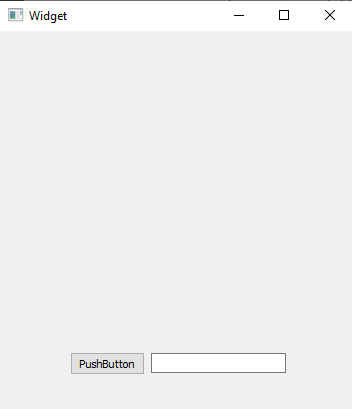
\includegraphics[width=0.4\textwidth]{./Figs/2021-05-03-23-19-04.png}
\end{itemize}

%----------------------------------------------------------------------------------------


